% !TEX root = ../notes_template.tex
\chapter{Human Genome}\label{chp:human_genome}

\minitoc

\section{Introduction}
\begin{itemize}
    \item 3.2 billion base pairs 
    \item Haploid (n, gametes): 22 autosomal chromosomes + 1 sexual (X or Y).
    \item Diploid (2n, zygote): 46 autosomal chromosomes + 2 sexual (XX, XY). Every gene present in autosomes is present 
    in two copies in the zygote. Then individuals contain two genomes, one maternal and one paternal, which get mixed in 
    the cell nucleus after the first mitotic division.
    \item The total number of protein-coding genes distributed on the 23 chromosomes of the human genome is estimated to 
    be 20,412, slightly less than 20,470 genes of the \textit{Caenorhabditis elegans} \cite{Pena2021} and only the double of one strain of 
    \textit{Ktedonobacter racemifer}, with 11,453 protein-coding genes \cite{He2024}.
\end{itemize}
\begin{figure}[!ht]
    \centering
    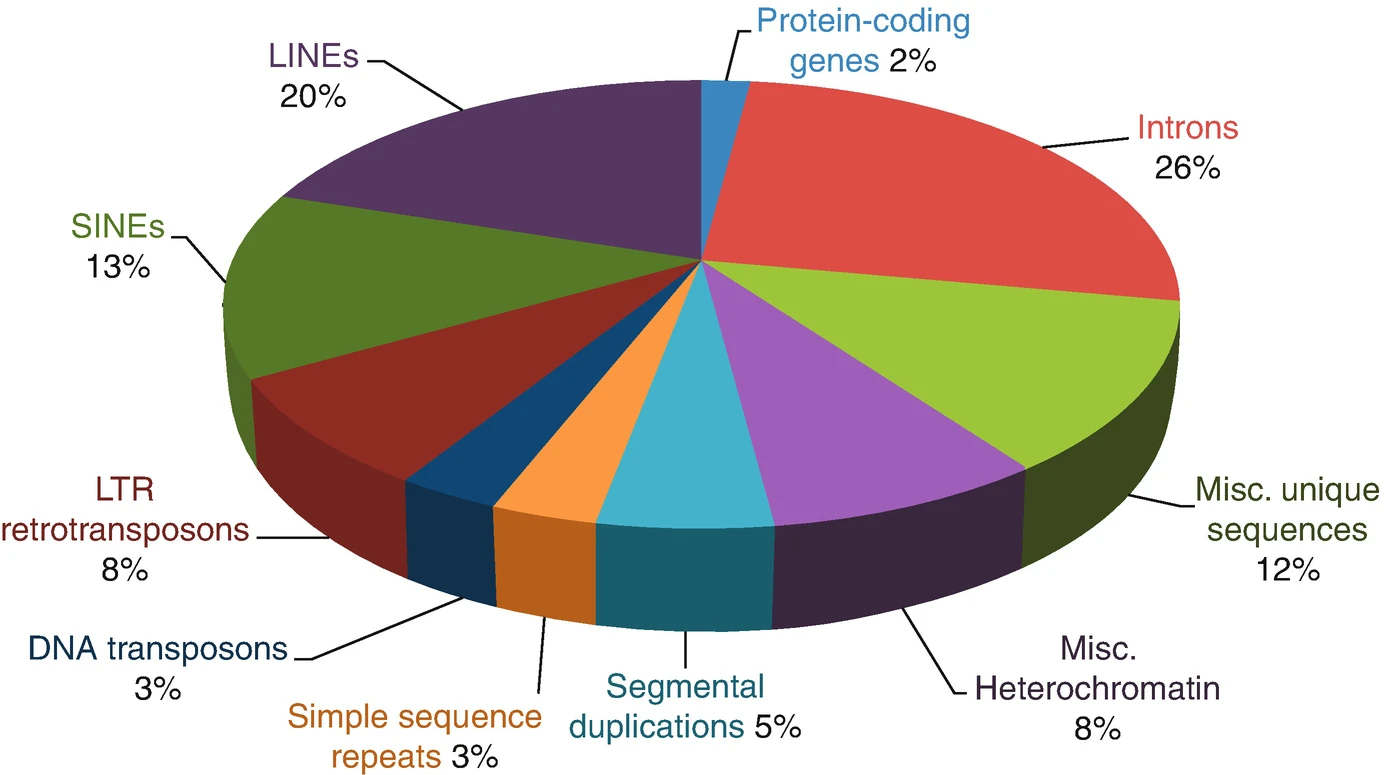
\includegraphics[width=1\linewidth]{./figure/composition_human_genome.png}
    \caption{Composition of the human genome. Redrawn from a graph that was produced in 2014 by the NHS National Genetics 
    and Genomics Education Centre. Borrowed from \citetitle{Pena2021} \cite{Pena2021}}
    \label{fig:composition_human_genome}
\end{figure}

\section{Chromosomes}

Chromosomes are the basic morphological division of the human genome.The number of genes on each human chromosome varies widely, 
from 2058 genes on chr1 to only 71 genes on Y chr. The density of genes on chromosomes also varies widely. For instance, 
chromosome 19 is smaller than chromosome 13, but contains almost four times more genes than the latter 
(chromosome 19 is the second in decreasing order of gene content, just behind the chromosome 1). The three autosomes 
with the fewest genes are chromosome 13 (327 genes), chr 18 (270 genes), and chr 21 (234 genes). It is thus no accident 
that the only autosomal human trisomies compatible with the survival of the fetus till birth are trisomies 13, 18 and 21! 

There is apparently no specific reason why humans have 46 chromosomes in somatic cells. Our closest primate, the chimpanzee 
(\textit{Pan troglodytes}) has 48 chromosomes. In the evolution of primates, two acrocentric chromosomes from the chimpanzee underwent 
centric fusion to form human chromosome 2, hence the reduction of chromosome number to 46. In contrast, the mouse (\textit{Mus musculus}) 
has 56 chromosomes. The \textit{Lysandra atlantica} butterfly has 446 chromosomes in diploid cells, while \textit{Lysandra golga} has 268 and 
\textit{Lysandra nivescens} has 82! In fact, there seems to be no correlation between the number of chromosomes or the size of the 
total genome or the biological complexity of the species. Both seem to vary at random. Thus, everything suggests that the 
chromosomes may be only physical frameworks that allow the realization of mitosis and meiosis in sexual species. 

The chromosomes seem to behave functionally as “packages” of genes. In general, the functioning of individual genes is not 
affected by their chromosomal position. For instance, there are individuals with balanced chromosomal translocations, in 
which chromosomes have exchanged segments without loss or net gain of genetic material—such individuals do not present any 
clinical manifestation of translocation, except perhaps for reproductive difficulties, as some translocations may interfere 
with the production of gametes in meiosis, especially in the male. 

\textbf{Centromere}. In chromosomes, DNA contains genes that are expressed according to the needs of the cell, but it also contains 
specialized sequences that are necessary for intrinsic functions of the chromosome itself. On one hand, chromosomes need 
to be properly aligned during cell division. This requires a centromere, a region where a pair of protein complexes, called 
kinetochores, binds just before the start of cell division. Microtubules are responsible initially for positioning the 
chromosomes correctly in the metaphase and then for pulling the individualized chromosomes to opposite poles of the mitotic 
spindle. The DNA sequences in the centromeres are very different in different organisms. In mammalian chromosomes, centromeric 
DNA is a heterochromatic region, with no informational content, dominated by repetitive DNA sequences that often extend 
monotonously by mega DNA bases. 

\textbf{Telomere}. At the ends of chromosomes, there are specialized structures called telomeres, which are necessary for maintaining 
chromosomal integrity. If a telomere is lost after a break in a chromosome, the resulting chromosomal end is unstable and 
tends to merge with the broken ends of the other chromosomes, or even be degraded. In vertebrate telomeres the DNA consists 
of multiple copies in tandem of the oligonucleotide TTAGGG, sequence at which certain telomeric proteins bind. The repetitive 
units of the telomeres decrease in number with every division of the DNA. As the enzyme needed to regenerate telomeres (telomerase) 
is not available in normal somatic cells, telomeres are a kind of biological clock that records our age.  

\section{Coding and Non-coding DNA}
The vast majority of genes are in the chromosomes of the nucleus; a few are also found in mitochondrial DNA. 

\textbf{Human vs Chimpanzee}. Remarkable similarities of known human and chimpanzee protein sequences initially led to the 
suggestion that significant differences might be primarily in gene and protein expression, rather than protein structure. 
Further analysis of alignable non-coding sequences affirmed this \(\backsim\)1\% difference. However, the subsequent identification 
of non-alignable sequences that were due to segmental deletions and duplications has shown that the overall difference between 
the two genomes is actually \(\backsim\)4\%.  

Less than 2\% of the human genome corresponds to protein-coding genes (\autoref{fig:composition_human_genome}). The functional 
role of the remaining 98\%, apart from repetitive sequences (constitutive heterochromatin) that appear to have a structural 
role in the chromosome, is a matter of controversy. 

\section{Retroposons, Retrotransposons, and Retrovirus}
Transposable elements can be separated into two major classes: 
\begin{itemize}
    \item \textbf{DNA transposons}. Constitute approximately 3\% of the human genome (\autoref{fig:composition_human_genome}; 
    \autoref{fig:human_transposable_elements}), 
    can excise themselves from the genome, move as DNA and insert themselves into new genomic sites. Although DNA transposons 
    are currently not mobile in the human genome, they were apparently active during early primate evolution.
    \item \textbf{Retroposition elements}. i.e. retroposons, retrotransposons and endogenous retroviruses, duplicate through 
    RNA intermediates that are reverse transcribed and inserted at new genomic locations. Together, they constitute more 
    than 40\% of the human genome.
\end{itemize}
\begin{figure}[!ht]
    \centering
    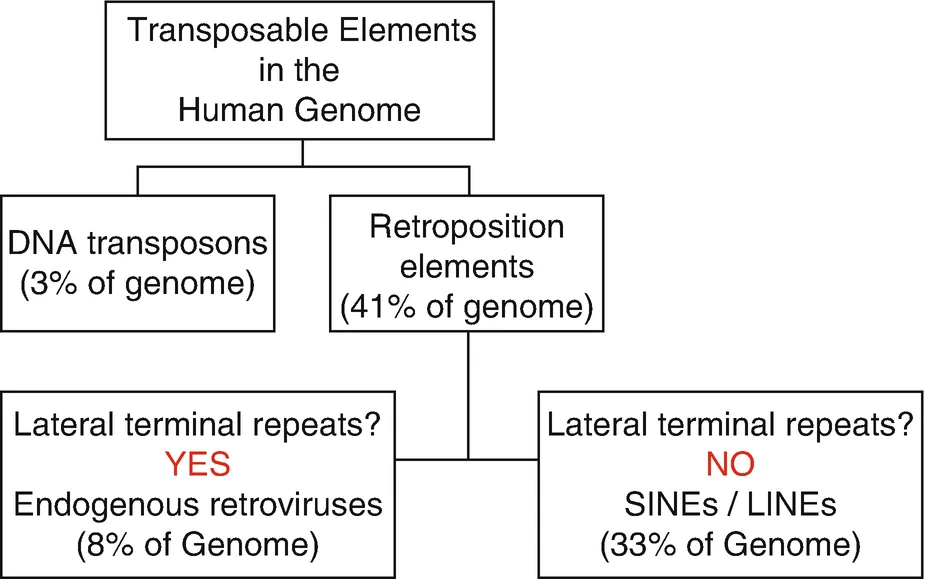
\includegraphics[width=1\linewidth]{./figure/human_transposable_elements.png}
    \caption{Classes of transposable elements in the human genome. Borrowed from \citetitle{Pena2021} \cite{Pena2021}}
    \label{fig:human_transposable_elements}
\end{figure}

\textbf{Retroposons}. Do not contain the gene for reverse transcriptase and thus are dependent on exogenous sources of 
the enzyme (mostly from Long Interspersed Nuclear Element s—LINEs) for retroposition. They share similarity with genes 
transcribed by RNA polymerase III, the enzyme that transcribes genes into ribosomal RNA, tRNA and other small RNA molecules. 
An especially abundant group of retroposons in humans is the Alu family of SINEs (Short Interspersed Nuclear Elements ), 
that basically represents a processed pseudogene of the Signal Recognition Particle (7SL) RNA. The Alu family of retroposons 
(thus called because they contain a site for digestion by the restriction enzyme AluI) makes up 13\% of the human genome. 
Virtually all other mammalian SINEs differ from the human, being derived from tRNA genes.  

\textbf{Retrotransposons}. In contrast, do code for reverse transcriptase and hence are capable of autonomous retrotranscription. 
They also contain a promoter for RNA polymerase II, which allows it to insert itself into random positions. In humans, LINEs, 
which altogether make up 20\% of the human genome, are the main class of retrotransposons. Although the vast majority of 
human LINE-1 sequences are inactive molecular fossils, an estimated 80-100 copies per individual still retain the ability 
to mobilize and expand in numbers within the human genome, by cycles of transcription, retrotranscription and retroposition. 
Some of these active LINEs constitute insertional polymorphisms in the human species. LINEs and SINEs continue growing in 
numbers in all mammalian genomes, and thus are “genomic parasites”, the ultimate “selfish genes”.  

\textbf{Endogenous retroviruses}. The class of retrotransposons that contain lateral terminal repeats (LTRs), which are evolutionarily 
related to the exogenous retrovirus group of RNA virus and will be the focus of this section (\autoref{fig:human_transposable_elements}). 
They constitute around 8\% of the human genome! This is ironic, considering that at the very moment that I am writing this 
chapter humanity is being held ransom by the RNA virus SARS-CoV-2 that causes the serious disease COVID-19. Thus, if not 
only for its timeliness, I think that today any discussion of the structure and function of the human genome should include 
a discussion of these endogenous retroviruses. In special I want to evaluate the evidence for a conceivable anti-viral effect 
of these mostly defective and dormant endogenous retroviruses, which eons ago were exogenous, infected germ cells, endogenized 
and multiplied to become 8\% of the human genome. 

An endogenous retrovirus is generally called ERV or EVE (endogenous viral element). Although not one of the thousands of 
retrovirus-related sequences found in the human genome contains a complete set of intact retroviral genes or can express 
infectious virus, these sequences are nonetheless referred to as Human Endogenous Retroviruses (HERVs). More info in the 
section of An Overview of the Human Genome.